\documentclass[12pt]{article}
\usepackage[a4paper, total={5.5in, 9in}]{geometry}
\usepackage{amsmath}
\usepackage{amsfonts}
\usepackage{graphicx}
\usepackage{pgfplots}
\pgfplotsset{compat=1.18}
\usepackage{enumitem}

\title{College Algebra Worksheet 5.2}
\author{PCL Learning Center}
\date{}

\begin{document}
\maketitle

\begin{center}
    \textit{note: No graphing calculators or electronic devices may be used on this worksheet.}    
\end{center}

\section*{Problem Set 1\\Difficulty level: Normal}
\subsection*{Problem 1}
Which set of words describes the end behavior of the following function?
\[f(x)=0.4(2x-9)(3x+1)(x-7)(x+9)\]
\begin{enumerate}[label=(\alph*)]
    \item rising as $x$ approaches negative and positive infinity.
    \item falling as $x$ approaches negative and positive infinity.
    \item rising as $x$ approaches negative infinity and falling as $x$ approaches positive infinity.
    \item falling as $x$ approaches negative infinity and rising as $x$ approaches positive infinity.
\end{enumerate}

\subsection*{Problem 2}
Which of the following shows the graph of a polynomial function?
\begin{enumerate}[label=(\alph*)]
    \item
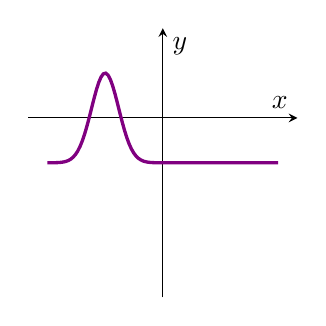
\begin{tikzpicture}
\begin{axis}[
    axis lines=middle,
    width=5cm,
    height=5cm,
    xmin=-7, xmax=7,
    ymin=-2, ymax=1,  % Adjusted y-limits
    grid=both,
    xlabel=$x$,
    ylabel=$y$,
    xtick=\empty,
    ytick=\empty,
    minor tick num=1,
    restrict y to domain=-10:10  % Added restriction
]
\addplot[domain=-6:6, samples=100, very thick, violet] {exp(-(x+3)^2)-0.5};
\end{axis}
\end{tikzpicture}

    \item
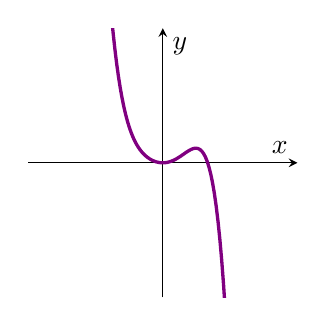
\begin{tikzpicture}
\begin{axis}[
    axis lines=middle,
    width=5cm,
    height=5cm,
    xmin=-3, xmax=3,  % Reduced x-range
    ymin=-3, ymax=3,  % Reduced y-range
    grid=both,
    xlabel=$x$,
    ylabel=$y$,
    xtick=\empty,
    ytick=\empty,
    minor tick num=1,
    restrict y to domain=-10:10  % Added restriction
]
\addplot[domain=-2:2, samples=100, very thick, violet] {-x^5+x^2};
\end{axis}
\end{tikzpicture}

    \item
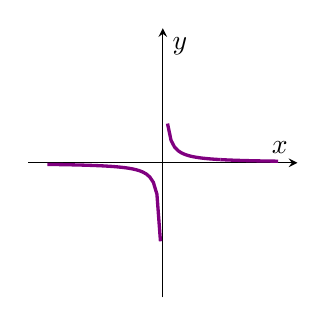
\begin{tikzpicture}
\begin{axis}[
    axis lines=middle,
    width=5cm,
    height=5cm,
    xmin=-7, xmax=7,
    ymin=-7, ymax=7,
    grid=both,
    xlabel=$x$,
    ylabel=$y$,
    xtick=\empty,
    ytick=\empty,
    minor tick num=1,
    restrict y to domain=-7:7  % Added restriction
]
\addplot[domain=-6:3, samples=50, very thick, violet] {1/(2*x)};
\addplot[domain=3:6, samples=50, very thick, violet] {1/(2*x)};
\end{axis}
\end{tikzpicture}

    \item
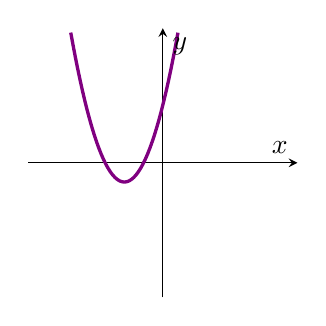
\begin{tikzpicture}
\begin{axis}[
    axis lines=middle,
    width=5cm,
    height=5cm,
    xmin=-7, xmax=7,
    ymin=-7, ymax=7,
    grid=both,
    xlabel=$x$,
    ylabel=$y$,
    xtick=\empty,
    ytick=\empty,
    minor tick num=1,
    restrict y to domain=-7:7  % Added restriction
]
\addplot[domain=-6:6, samples=100, very thick, violet] {(x+2)^2-1};
\end{axis}
\end{tikzpicture}
\end{enumerate}

\subsection*{Problem 3}
Which of the following is a polynomial function? Select all that apply.

    \begin{enumerate}
        \item[(a)] \(4 \cdot 11^x\)
        \item[(b)] \(3 \cdot 18^x\)
        \item[(c)] \(10 \cdot 17^x\)
        \item[(d)] \(-4x^3-4x^2+5x+1\)
        \item[(e)] \(-2x-1\)
    \end{enumerate}

\subsection*{Problem 4}
Which of the following is a power function? Select all that apply.

    \begin{enumerate}
        \item[(a)] \(5 \cdot 3^x\)
        \item[(b)] \(5 \cdot 14^x\)
        \item[(c)] \(\sqrt[6]{x}\)
        \item[(d)] \(2 \cdot 14^x\)
        \item[(e)] \(\dfrac{5}{x^9}\)
    \end{enumerate}

\subsection*{Problem 5}
Which factor could be part of the function so that \(f(x)\) decreases as \(x\) approaches infinity and as \(x\) approaches negative infinity? Select all that apply.
\[f(x)=(3x+1)(2x-5)(x+9)(?)\]

    \begin{enumerate}
        \item[(a)] \(-4\)
        \item[(b)] \(-\dfrac{2}{3}x\)
        \item[(c)] \(5x^2\)
        \item[(d)] \(3x-7\)
        \item[(e)] \(-(x^3+4)\)
    \end{enumerate}

\subsection*{Problem 6}
Which function shows \(f(x)\) decreasing as \(x\) approaches negative and positive infinity? Select all that apply.

    \begin{enumerate}[label=(\alph*)]
    \item $\ f(x) = 2x(3x + 1)(2x - 5)$
    \item $\ f(x) = -\dfrac{2}{3}(3x + 1)(2x + 5)$
    \item $\ f(x) = -5x(2x + 1)(x + 9)(x - 3)$
    \item $\ f(x) = -\dfrac{1}{3}x^3(4x + 3)(2x + 7)(x + 5)(x + 2)$
    \item $\ f(x) = 9x^3(2x - 3)(3x + 5)(x + 2)(x - 3)$
\end{enumerate}

\subsection*{Problem 7}
Is the following a power function, a polynomial, both, or neither?
\[f(x)=-17x^5\]

\subsection*{Problem 8}
For the following exercises, identify the function as a power function, a polynomial function, or neither.

    \begin{enumerate}[label=(\alph*)]
    \item $f(x) = x^5$
    \item $f(x) = (x^2)^3$
    \item $f(x) = x - x^4$
    \item $f(x) = \dfrac{x^2}{x^2-1}$
    \item $f(x) = 2x \left( x + 2 \right) \left( x - 1 \right)^2$
    \item $f(x) = 3^{x+1}$
    \end{enumerate}

\section*{Problem Set 2\\Difficulty level: Hard}
\subsection*{Problem 1}
For the following exercises, determine the end behavior of the functions.

    \begin{enumerate}[label=(\alph*)]
    \item $f(x) = -2x^4 - 3x^2 + x - 1$
    \item $f(x) = 3x^2 + x - 2$
    \item $f(x) = x^2 \left( 2x^3 - x + 1 \right)$
    \item $f(x) = (2 - x)^7$
    \end{enumerate}

\newpage
\section*{Solutions to the Set 1}
\subsection*{Problem 1}
\begin{enumerate}[label=(\alph*)]
    \item rising as $x$ approaches negative and positive infinity.
\end{enumerate}
\subsection*{Problem 2}
\begin{enumerate}
    \item[(b)]
    \item[(d)]
\end{enumerate}
\subsection*{Problem 3}
\begin{enumerate}
    \item[(d)] \(-4x^3-4x^2+5x+1\)
    \item[(e)] \(-2x-1\) 
\end{enumerate}
\subsection*{Problem 4}
\begin{enumerate}
        \item[(c)] \(\sqrt[6]{x}\)
        \item[(e)] \(\dfrac{5}{x^9}\)
\end{enumerate}
\subsection*{Problem 5}
\begin{enumerate}
    \item[(b)] $\ f(x) = -\dfrac{2}{3}(3x + 1)(2x + 5)$
    \item[(e)] $\ f(x) = 9x^3(2x - 3)(3x + 5)(x + 2)(x - 3)$
\end{enumerate}
\subsection*{Problem 6}
\begin{enumerate}
    \item[(b)] $\ f(x) = -\dfrac{2}{3}(3x + 1)(2x + 5)$
    \item[(c)] $\ f(x) = -5x(2x + 1)(x + 9)(x - 3)$ 
\end{enumerate}
\subsection*{Problem 7}
Both power and polynomial.
\subsection*{Problem 8}
    \begin{enumerate}[label=(\alph*)]
    \item Power
    \item Power
    \item Polynomial
    \item Neither
    \item Polynomial
    \item Neither
    \end{enumerate}
\section*{Solutions to the Set 2}
\subsection*{Problem 1}

    \begin{enumerate}
        \item[(a)] Falls both sides
        \item[(b)] Rises both sides
        \item[(c)] Falls left, rises right
        \item[(d)] Rises left, falls right
    \end{enumerate}

\end{document}